\newpage 
\section{Experiments}

In this section we present experimental data on the performance of Algorithm \ref{alg}. We also compare its performance to an algorithm that uses the full gradient information.

We consider a time-varying least-squares problem of the form:

$$\min_{x\in \mathcal{B}} \frac{1}{2} \norm{Ax-b_t}^2$$

where $\mathcal{B}$ is the unit ball, $A \in \mathbb{R}^{n \times d}$ is a given regression matrix, and $b_t$ is a time-varying vector. We now outline how the loss functions $\lt = \frac{1}{2} \norm{Ax-b_t}^2$ are generated.

We generate $A$ by defining its singular value decomposition: for its left and right-singular vectors, sample two orthogonal matrices $U \in \mathbb{R}^{n \times n}$ and $V \in \mathbb{R}^{d \times d}$. Then we let the singular values be equally spaced from $1/\sqrt{\kappa}$ to $1$. We consider $\kappa = 100$. 

We generate $b_t$ with
$$b_t = A \xst+ w_t$$

where $\xst$ is generated using a random walk with step size of $1$ ($\norm{\xst - x_{t-1}^*} = 1 ~~ \forall t$) and $w_t$ is a zero-mean Gaussian vector with covariance matrix $10^{-3}I_n$. Hence $\sumt \norm{\xst - x_{t-1}^*} = T$.

Clearly the $\lt$'s are $\mu$-strongly convex and $L$-smooth with $\mu = 1/\sqrt{\kappa}$ and $L \leq \norm{A} = 1$. We also have that $\lt$ is $G$-Lipschitz with $G = 6 \norm{A^\intercal A}^2 = 6$. 


\begin{figure}[hbt!]\centering
    \subfloat{
    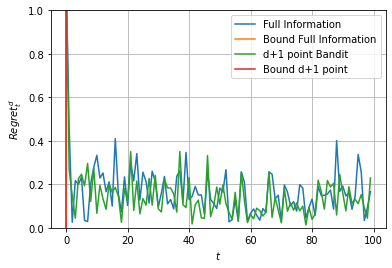
\includegraphics[width=0.45\linewidth]{fig1.png}}\hfill
	\subfloat{
	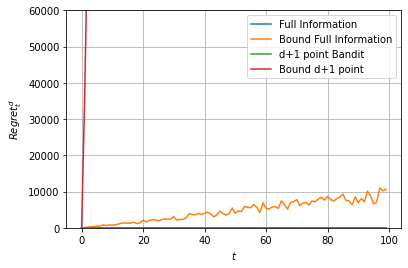
\includegraphics[width=0.45\linewidth]{fig2.png}}
    \caption{Plot showing the regret of Algorithm \ref{alg} and the full-information OGD along with bounds for both. Note that both the bounds diverge almost immediately.}
    \label{fig:exp}
\end{figure}




